\documentclass{standalone}
\usepackage{tikz}
\usepackage{pgfplots}
\pgfplotsset{compat=newest}
\usepackage{amsmath}
\usepackage[american]{circuitikz}
\usepackage{cmbright}

\definecolor{myred}{RGB}{170,0,0}
\definecolor{myblue}{RGB}{0,0,220}
\definecolor{mygreen}{RGB}{0,150,0}
\definecolor{myorange}{RGB}{255,127,0}
\definecolor{mybrown}{RGB}{150,75,0}

\begin{document}
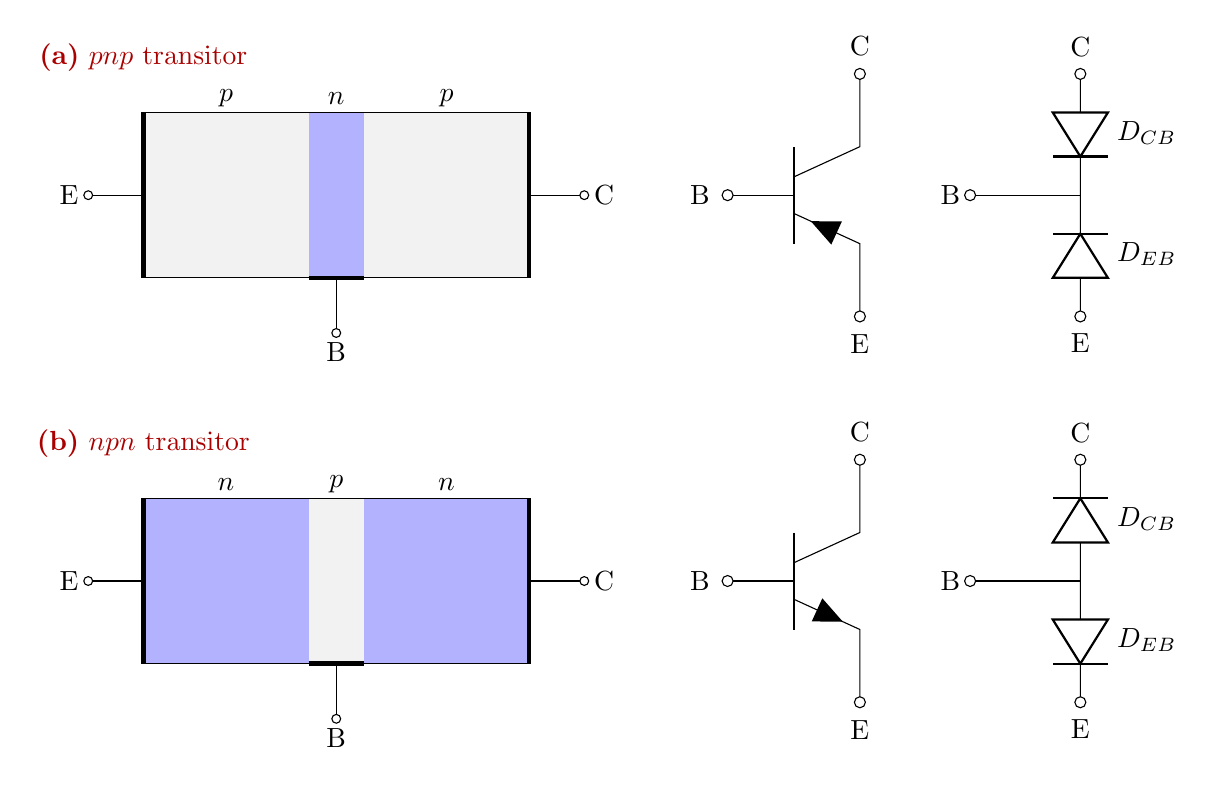
\begin{tikzpicture}
    \begin{scope}[scale=0.7]
        % Title
        \node[anchor=center, color=myred] at (0, 4.0) {\textbf{(a)} $pnp$ transitor};
        % Regions
        % n-region
        \fill[gray!10] (0,0) rectangle (3,3);
        % n-region
        \fill[blue!30] (3,0) rectangle (4,3);
        % n-region
        \fill[gray!10] (4,0) rectangle (7,3);
        \draw[thin, black] (0, 0) rectangle (7, 3);

        % Line at the interface.
        % \draw[thin, black] (4, 3) -- (4, 0);

        % Metal contact lines
        \draw[ultra thick, black] (0,3) -- (0,0);
        \draw[ultra thick, black] (7,3) -- (7,0);
        \draw[ultra thick, black] (3,0) -- (4,0);
        \draw[thin, black] (-1, 1.5) -- (0, 1.5);
        \draw[thin, black] (7, 1.5) -- (8, 1.5);
        \draw[thin, black] (3.5, 0) -- (3.5, -1);

        % Contact terminals.
        \draw (-1, 1.5) node[ocirc] (E) {};
        \draw (8, 1.5) node[ocirc] (C) {};
        \draw (3.5, -1) node[ocirc] (B) {};

        % Labels
        \node[anchor=center, color=black] at (1.5, 3.25) {$p$};
        \node[anchor=center, color=black] at (3.5, 3.25) {$n$};
        \node[anchor=center, color=black] at (5.5, 3.25) {$p$};
        \node [anchor=east, color=black] at (-1, 1.5) {E};
        \node [anchor=west, color=black] at (8, 1.5) {C};
        \node [anchor=north, color=black] at (3.5, -1) {B};

        % pnp BJT sumbol
        \draw (13, 1.5) node[pnp, scale=2.0, yscale=-1] (Q) {};
        \node[ocirc, scale=1.25] (Q1E) at (Q.E) {};
        \node at ([yshift=-0.5cm]Q1E) {E};
        \node[ocirc, scale=1.25] (Q1C) at (Q.C) {};
        \node at ([yshift=0.5cm]Q1C) {C};
        \node[ocirc, scale=1.25] (Q1B) at (Q.B) {};
        \node at ([xshift=-0.5cm]Q1B) {B};

        % Double diode model
        \draw (17, -0.7) to[diode, l_=$D_{EB}$] (17, 1.5);
        \node[ocirc, scale=1.25] (D1E) at (17, -0.7) {};
        \node [anchor=north, color=black] at (17, -0.84) {E};
        \draw (17, 1.5) to[diode, l_=$D_{CB}$, invert] (17, 3.7);
        \node[ocirc, scale=1.25] (D1E) at (17, 3.7) {};
        \draw (15, 1.5) -- (17, 1.5);
        \node[ocirc, scale=1.25] (D1E) at (15, 1.5) {};
        \node [anchor=south, color=black] at (17, 3.84) {C};
        \node [anchor=east, color=black] at (15, 1.5) {B};
    \end{scope}
    
    \begin{scope}[scale=0.7, yshift=-7cm]
        % Title
        \node[anchor=center, color=myred] at (0, 4.0) {\textbf{(b)} $npn$ transitor};
        % Regions
        % n-region
        \fill[blue!30] (0,0) rectangle (3,3);
        % p-region
        \fill[gray!10] (3,0) rectangle (4,3);
        % n-region
        \fill[blue!30] (4,0) rectangle (7,3);
        \draw[thin, black] (0, 0) rectangle (7, 3);

        % Metal contact lines
        \draw[ultra thick, black] (0,3) -- (0,0);
        \draw[ultra thick, black] (7,3) -- (7,0);
        \draw[ultra thick, black] (3,0) -- (4,0);
        \draw[thin, black] (-1, 1.5) -- (0, 1.5);
        \draw[thin, black] (7, 1.5) -- (8, 1.5);
        \draw[thin, black] (3.5, 0) -- (3.5, -1);

        % Contact terminals.
        \draw (-1, 1.5) node[ocirc] (E) {};
        \draw (8, 1.5) node[ocirc] (C) {};
        \draw (3.5, -1) node[ocirc] (B) {};

        % Labels
        \node[anchor=center, color=black] at (1.5, 3.25) {$n$};
        \node[anchor=center, color=black] at (3.5, 3.25) {$p$};
        \node[anchor=center, color=black] at (5.5, 3.25) {$n$};
        \node [anchor=east, color=black] at (-1, 1.5) {E};
        \node [anchor=west, color=black] at (8, 1.5) {C};
        \node [anchor=north, color=black] at (3.5, -1) {B};

        % npn BJT sumbol
        \draw (13, 1.5) node[npn, scale=2.0] (Q) {};
        \node[ocirc, scale=1.25] (Q1E) at (Q.E) {};
        \node at ([yshift=-0.5cm]Q1E) {E};
        \node[ocirc, scale=1.25] (Q1C) at (Q.C) {};
        \node at ([yshift=0.5cm]Q1C) {C};
        \node[ocirc, scale=1.25] (Q1B) at (Q.B) {};
        \node at ([xshift=-0.5cm]Q1B) {B};

        % Double diode model
        \draw (17, -0.7) to[diode, l_=$D_{EB}$, invert] (17, 1.5);
        \node[ocirc, scale=1.25] (D1E) at (17, -0.7) {};
        \node [anchor=north, color=black] at (17, -0.84) {E};
        \draw (17, 1.5) to[diode, l_=$D_{CB}$] (17, 3.7);
        \node[ocirc, scale=1.25] (D1E) at (17, 3.7) {};
        \draw (15, 1.5) -- (17, 1.5);
        \node[ocirc, scale=1.25] (D1E) at (15, 1.5) {};
        \node [anchor=south, color=black] at (17, 3.84) {C};
        \node [anchor=east, color=black] at (15, 1.5) {B};
    \end{scope}
\end{tikzpicture}
\end{document}